% Options for packages loaded elsewhere
% Options for packages loaded elsewhere
\PassOptionsToPackage{unicode}{hyperref}
\PassOptionsToPackage{hyphens}{url}
\PassOptionsToPackage{dvipsnames,svgnames,x11names}{xcolor}
%
\documentclass[
  french,
  letterpaper,
  DIV=11,
  numbers=noendperiod]{scrartcl}
\usepackage{xcolor}
\usepackage[margin=1.5cm]{geometry}
\usepackage{amsmath,amssymb}
\setcounter{secnumdepth}{-\maxdimen} % remove section numbering
\usepackage{iftex}
\ifPDFTeX
  \usepackage[T1]{fontenc}
  \usepackage[utf8]{inputenc}
  \usepackage{textcomp} % provide euro and other symbols
\else % if luatex or xetex
  \usepackage{unicode-math} % this also loads fontspec
  \defaultfontfeatures{Scale=MatchLowercase}
  \defaultfontfeatures[\rmfamily]{Ligatures=TeX,Scale=1}
\fi
\usepackage{lmodern}
\ifPDFTeX\else
  % xetex/luatex font selection
\fi
% Use upquote if available, for straight quotes in verbatim environments
\IfFileExists{upquote.sty}{\usepackage{upquote}}{}
\IfFileExists{microtype.sty}{% use microtype if available
  \usepackage[]{microtype}
  \UseMicrotypeSet[protrusion]{basicmath} % disable protrusion for tt fonts
}{}
\usepackage{setspace}
\makeatletter
\@ifundefined{KOMAClassName}{% if non-KOMA class
  \IfFileExists{parskip.sty}{%
    \usepackage{parskip}
  }{% else
    \setlength{\parindent}{0pt}
    \setlength{\parskip}{6pt plus 2pt minus 1pt}}
}{% if KOMA class
  \KOMAoptions{parskip=half}}
\makeatother
% Make \paragraph and \subparagraph free-standing
\makeatletter
\ifx\paragraph\undefined\else
  \let\oldparagraph\paragraph
  \renewcommand{\paragraph}{
    \@ifstar
      \xxxParagraphStar
      \xxxParagraphNoStar
  }
  \newcommand{\xxxParagraphStar}[1]{\oldparagraph*{#1}\mbox{}}
  \newcommand{\xxxParagraphNoStar}[1]{\oldparagraph{#1}\mbox{}}
\fi
\ifx\subparagraph\undefined\else
  \let\oldsubparagraph\subparagraph
  \renewcommand{\subparagraph}{
    \@ifstar
      \xxxSubParagraphStar
      \xxxSubParagraphNoStar
  }
  \newcommand{\xxxSubParagraphStar}[1]{\oldsubparagraph*{#1}\mbox{}}
  \newcommand{\xxxSubParagraphNoStar}[1]{\oldsubparagraph{#1}\mbox{}}
\fi
\makeatother


\usepackage{longtable,booktabs,array}
\usepackage{calc} % for calculating minipage widths
% Correct order of tables after \paragraph or \subparagraph
\usepackage{etoolbox}
\makeatletter
\patchcmd\longtable{\par}{\if@noskipsec\mbox{}\fi\par}{}{}
\makeatother
% Allow footnotes in longtable head/foot
\IfFileExists{footnotehyper.sty}{\usepackage{footnotehyper}}{\usepackage{footnote}}
\makesavenoteenv{longtable}
\usepackage{graphicx}
\makeatletter
\newsavebox\pandoc@box
\newcommand*\pandocbounded[1]{% scales image to fit in text height/width
  \sbox\pandoc@box{#1}%
  \Gscale@div\@tempa{\textheight}{\dimexpr\ht\pandoc@box+\dp\pandoc@box\relax}%
  \Gscale@div\@tempb{\linewidth}{\wd\pandoc@box}%
  \ifdim\@tempb\p@<\@tempa\p@\let\@tempa\@tempb\fi% select the smaller of both
  \ifdim\@tempa\p@<\p@\scalebox{\@tempa}{\usebox\pandoc@box}%
  \else\usebox{\pandoc@box}%
  \fi%
}
% Set default figure placement to htbp
\def\fps@figure{htbp}
\makeatother


% definitions for citeproc citations
\NewDocumentCommand\citeproctext{}{}
\NewDocumentCommand\citeproc{mm}{%
  \begingroup\def\citeproctext{#2}\cite{#1}\endgroup}
\makeatletter
 % allow citations to break across lines
 \let\@cite@ofmt\@firstofone
 % avoid brackets around text for \cite:
 \def\@biblabel#1{}
 \def\@cite#1#2{{#1\if@tempswa , #2\fi}}
\makeatother
\newlength{\cslhangindent}
\setlength{\cslhangindent}{1.5em}
\newlength{\csllabelwidth}
\setlength{\csllabelwidth}{3em}
\newenvironment{CSLReferences}[2] % #1 hanging-indent, #2 entry-spacing
 {\begin{list}{}{%
  \setlength{\itemindent}{0pt}
  \setlength{\leftmargin}{0pt}
  \setlength{\parsep}{0pt}
  % turn on hanging indent if param 1 is 1
  \ifodd #1
   \setlength{\leftmargin}{\cslhangindent}
   \setlength{\itemindent}{-1\cslhangindent}
  \fi
  % set entry spacing
  \setlength{\itemsep}{#2\baselineskip}}}
 {\end{list}}
\usepackage{calc}
\newcommand{\CSLBlock}[1]{\hfill\break\parbox[t]{\linewidth}{\strut\ignorespaces#1\strut}}
\newcommand{\CSLLeftMargin}[1]{\parbox[t]{\csllabelwidth}{\strut#1\strut}}
\newcommand{\CSLRightInline}[1]{\parbox[t]{\linewidth - \csllabelwidth}{\strut#1\strut}}
\newcommand{\CSLIndent}[1]{\hspace{\cslhangindent}#1}

\ifLuaTeX
\usepackage[bidi=basic]{babel}
\else
\usepackage[bidi=default]{babel}
\fi
% get rid of language-specific shorthands (see #6817):
\let\LanguageShortHands\languageshorthands
\def\languageshorthands#1{}


\setlength{\emergencystretch}{3em} % prevent overfull lines

\providecommand{\tightlist}{%
  \setlength{\itemsep}{0pt}\setlength{\parskip}{0pt}}



 


\KOMAoption{captions}{tableheading}
\usepackage{lineno}
\linenumbers
\renewcommand\thelinenumber{\arabic{linenumber}}
\setcounter{linenumber}{1}
\modulolinenumbers[5]
\usepackage{graphicx}
\usepackage{tabularx}
\usepackage{multirow}
\usepackage{geometry}
\makeatletter
\@ifpackageloaded{caption}{}{\usepackage{caption}}
\AtBeginDocument{%
\ifdefined\contentsname
  \renewcommand*\contentsname{Table des matières}
\else
  \newcommand\contentsname{Table des matières}
\fi
\ifdefined\listfigurename
  \renewcommand*\listfigurename{Liste des Figures}
\else
  \newcommand\listfigurename{Liste des Figures}
\fi
\ifdefined\listtablename
  \renewcommand*\listtablename{Liste des Tables}
\else
  \newcommand\listtablename{Liste des Tables}
\fi
\ifdefined\figurename
  \renewcommand*\figurename{Figure}
\else
  \newcommand\figurename{Figure}
\fi
\ifdefined\tablename
  \renewcommand*\tablename{Table}
\else
  \newcommand\tablename{Table}
\fi
}
\@ifpackageloaded{float}{}{\usepackage{float}}
\floatstyle{ruled}
\@ifundefined{c@chapter}{\newfloat{codelisting}{h}{lop}}{\newfloat{codelisting}{h}{lop}[chapter]}
\floatname{codelisting}{Listing}
\newcommand*\listoflistings{\listof{codelisting}{Liste des Listings}}
\makeatother
\makeatletter
\makeatother
\makeatletter
\@ifpackageloaded{caption}{}{\usepackage{caption}}
\@ifpackageloaded{subcaption}{}{\usepackage{subcaption}}
\makeatother
\usepackage{bookmark}
\IfFileExists{xurl.sty}{\usepackage{xurl}}{} % add URL line breaks if available
\urlstyle{same}
\hypersetup{
  pdftitle={Characterization and evolution of hourly extreme precipitation in France using an Explicit-Convection Regional Climate Model},
  pdflang={fr},
  colorlinks=true,
  linkcolor={blue},
  filecolor={Maroon},
  citecolor={Blue},
  urlcolor={Blue},
  pdfcreator={LaTeX via pandoc}}


\title{Characterization and evolution of hourly extreme precipitation in
France using an Explicit-Convection Regional Climate Model}
\author{Nicolas Decoopman, Juliette Blanchet (Univ. Grenoble Alpes, CNRS, INRAE,
IRD, Grenoble INP*, IGE, 38000 Grenoble, France), Antoine Blanc (RTM,
ONF, 38000 Grenoble, France}
\date{}
\begin{document}
\maketitle

\textbf{Abstract.} Climate change is intensifying the global water
cycle, with extreme precipitation events increasing in frequency and
intensity. While trends in daily precipitation extremes are
well-documented, sub-daily extremes---critical for flash flood
risk---remain poorly characterized, especially in France, due to limited
long-term, high-resolution observations. This study evaluates the
ability of the AROME regional climate model (2.5 km resolution,
1959--2022), forced by ERA5 reanalysis, to reproduce observed hourly
precipitation extremes and their trends, using a dense network of
Météo-France stations.

We first validate AROME's climatology against station data, showing that
the model accurately captures spatial patterns of precipitation
frequency, cumulative totals, and daily maxima, but systematically
underestimates hourly extremes, particularly in summer. Correlation with
observations is high for daily metrics (\emph{r} \textgreater{} 0.9) but
drops for hourly maxima (\emph{r} = 0.6--0.7), reflecting challenges in
resolving convective processes at 2.5 km resolution.

Using extreme value theory (GEV modeling), we then analyze trends in
10-year return levels for both daily and hourly extremes. At the daily
scale, AROME reproduces observed positive trends in southeastern France
(e.g., +20--30\% in the Mercantour and Rhône Valley), consistent with
previous studies and Clausius--Clapeyron scaling. At the hourly scale,
trends are more heterogeneous and less robust, with significant
increases in February, March, and November, but high spatial variability
and low model-observation correlation in summer. Filtering for
statistically significant trends improves agreement, especially in
winter and late autumn, but hourly extremes remain poorly captured in
spring and summer.

Our results highlight the added value of explicit-convection models for
extreme precipitation studies, while underscoring their limitations for
convective extremes at resolutions coarser than 1 km. The Rhône Valley
emerges as a hotspot for intensifying hourly extremes, driven by
increased moisture flux and orographic enhancement. This work provides
the first national-scale assessment of hourly precipitation trends in
France, offering new insights for flood risk management and climate
adaptation strategies.

\textbf{Keywords.} Extreme precipitation, climate change,
convection-permitting model, AROME, sub-daily trends, France, extreme
value theory, flash floods, Clausius--Clapeyron scaling

\section{Introduction and context}\label{introduction-and-context}

\textbf{Climate change} is driving a warming of the planet's surface
air, with a more pronounced increase over land than over oceans (IPCC
2021). Global warming has reached +1.1°C worldwide, +1.7°C in
metropolitan France, and +2°C in the French Alps compared to the
pre-industrial era. Furthermore, the Clausius-Clapeyron relation
indicates that warmer air can hold more moisture (+7\% per °C)
(Clapeyron 1834). Due to buoyancy (Archimedes' principle), warm air
surrounded by cooler air tends to rise. As warm air ascends in the
atmosphere, it undergoes adiabatic cooling, leading to the condensation
of water vapor and the formation of precipitation (Météo-France 2010).
However, under calm conditions, the central portion of the precipitation
distribution does not fully capitalize on this excess moisture.
Energetic constraints (radiative balance, evaporation, ocean-air
exchanges) and dynamic constraints (subsidence, synoptic winds) limit
the increase in mean precipitation to only 1--3\% per °C (IPCC 2021). In
contrast, during intense convective events (thunderstorms, rapid
cyclogenesis), rapid ascent condenses nearly all of this surplus,
causing short-duration extreme rainfall to increase by 5--8\% per
°C---almost matching the theoretical potential. Extreme precipitation
closely follows the Clausius-Clapeyron scaling, whereas mean rainfall
remains influenced by numerous other energetic and dynamic factors
(O'Gorman 2015). Thus, climate warming theoretically leads to an
increase in extreme precipitation, though this increase varies with
changes in atmospheric circulation and can be locally amplified (J.
Blanchet, Blanc, et Creutin 2021).

\textbf{Extreme precipitation events} are defined as intense rainfall
over short durations (1 hour to 24 hours), corresponding to the upper
tail of the precipitation intensity distribution. There is no consensus
on what constitutes an ``extreme'' event. Some authors study
precipitation intensities above the 99th percentile or seasonal/annual
maxima, while others define extreme precipitation as events rarely or
never encountered in a human lifetime (e.g., precipitation levels
expected once every 10, 20, or 50 years). Extreme events are at the
heart of climate and societal concerns, as they account for the majority
of costs associated with flooding, landslides, and infrastructure
failures (IPCC 2022). In 2024, numerous such events made headlines,
including in Nepal, Afghanistan, Central Europe, eastern Spain, and
France (World Meteorological Organization (WMO) 2025). Notably, in June
2024, intense high-altitude rainfall contributed to major flooding in
the Écrins massif (Blanc et al. 2024); in October 2024, over 600 mm of
rain in 48 hours caused widespread flooding in the Ardèche department
(Météo-France 2024a); and in May 2025, extremely intense but short-lived
thunderstorms (locally exceeding 120 mm/h) caused extensive damage in
southern Var (Météo-France 2025).

\textbf{Daily precipitation extremes} have increased in intensity and
frequency across more than half of the world's land regions, at a rate
close to +7\% per °C of warming (IPCC 2021). Some regional studies
suggest similar trends in a significant proportion of land areas Markus
G. Donat et al. (2016). In France, however, signals are far more
heterogeneous and less pronounced than for temperature, with strong
regional variations. In most regions, trends remain weak or
non-significant, and only in certain areas---particularly the
southeast---are clear signals detected. In this region, the frequency of
extreme Mediterranean episodes (cumulated rainfall \textgreater{} 200 mm
in 24 hours) has doubled between 1961 and 2020, although interannual
variability remains high (Météo‑France 2024). The mean intensity of
daily extremes has increased by +22\% between 1961 and 2015 (Ribes et
al. 2019). At the national scale, no significant trend was detectable in
annual maxima of daily precipitation until the 1990s. Since then, some
studies report increases of +20\% to +40\%, though these estimates
remain sensitive to the period and analytical method (Markus G. Donat et
al. 2016). In the southeastern Alps, the increase in 20-year return
level daily precipitation in autumn (1958--2017) could reach an order of
magnitude comparable to its mean value (\textasciitilde+100\%) (J.
Blanchet, Blanc, et Creutin 2021). Projections indicate that a +4°C
warming scenario could lead to an average increase of
\textasciitilde+15\% in daily extreme rainfall across France, and up to
+20\% in the northern half (Soubeyroux et al. 2025). There remains
strong spatial and interannual variability (IPCC 2021).

\textbf{Hourly extremes}, measured at 1-hour or shorter time steps, are
essential for characterizing intense convective phenomena (thunderstorm
downpours, stationary thunderstorms) often responsible for flash floods.
Due to the lack of long, spatially dense time series, there is no
systematic global analysis of sub-daily trends; available data are often
sparse, short, and non-significant. Nevertheless, several regional
studies detect an intensification of hourly extremes across nearly all
continents, though global confidence in an overall increase remains very
low (IPCC 2021). Increases in extreme rainfall have been observed in the
United States, China (summer), Australia (annually), South Africa
(summer), India, Malaysia, and Italy. Depending on the method and
region, studies highlight sensitivities ranging from +7\% to +13\% per
°C---up to twice the Clausius-Clapeyron rate (Molnar et al. 2015). In
France, few regional studies explicitly characterize this increase in
hourly extremes. Observed maximum 1-hour values now reach 40--60 mm
during major Mediterranean events, compared to 30--40 mm in the
1980s--1990s (Météo‑France 2024). Only the study by Berghald et al.
(2025) appears to quantify trends in hourly extremes in the Alps.
However, trends in hourly return levels remain weak to non-significant,
with no clear spatial or seasonal coherence, contrasting with the robust
signals observed at daily time scales. This suggests that hourly
extremes do not yet show a clear climate signal (Soubeyroux et al.
2015).

\textbf{The climatological observation network} developed in the late
19th century relied on manual readings, typically once per day (around 6
UTC, which still often defines the meteorological day). A nationwide
network became available from the 1950s--1960s, when coverage became
sufficiently dense. Hundreds of precipitation time series exist today
(Météo-France 2020). At the hourly scale, the first operational
automatic stations (SATIN) date back to 1967. The generalization and
modernization of the real-time network occurred primarily with RADOME
from 1996 onward, making hourly accumulations widely available and
disseminated from the 1990s--2000s. Today, the national radar mosaic
provides 5-minute data at 1-km resolution, publicly accessible in
archives. ANTILOPE rainfall fields (radar + rain gauges) are
operationally produced at a 15-minute resolution since 2017.

\textbf{Climate model simulations} of precipitation provide: 1) data
preceding the observed record (pre-1990); and 2) spatially complete and
physically consistent fields, particularly useful in poorly instrumented
areas. Global Circulation Models (GCMs) were not suitable for this
study, as convection is parameterized, leading to over-smoothed and
poorly located hourly precipitation at resolutions of 12--200 km. The
emergence of regional climate models with explicit convection (CPMs,
Convection-Permitting Models) offers a unique opportunity: they
realistically simulate the dynamics of intense precipitation at fine
spatial and temporal scales over long periods. For this study, the model
must be a Regional Climate Model (RCM, 1--4 km) with explicit convection
(CPM) to explicitly represent the initiation, organization, and
propagation of convective systems and their hourly extremes. Models
meeting these criteria include: WRF (3 km), COSMO-CLM (2.8 km),
AROME-Climate (2.5 km) (CNRM--Météo‐France 2007), ICON-LEM (2.5 km),
UKCP CPM (2.2 km), CP4-Africa, and ensembles such as
EURO-CP/FPS-Convection. A CP-RCM must be initialized (3D fields of
temperature, humidity, pressure, wind, etc.) and laterally forced.
Historically, these forcings used ERA-Interim (80 km / 6h / 1979--2019),
now replaced by ERA5 (25--31 km / 1h / 1949--present), which dynamically
drives a high-resolution regional model. As ERA5 is a reanalysis, the
regional model it forces aims to reconstruct past hourly weather
conditions, rather than producing prospective or stochastic climate
simulations. This approach allows, for example, the characterization of
convective environments (Copernicus Climate Change Service (C3S) et
European Centre for Medium-Range Weather Forecasts (ECMWF) 2025), which
can then be refined using a CPM to explicitly simulate convection. The
AROME model (Application of Research to Operations at MEsoscale, 2.5 km
/ 1h), forced by ERA5 over the period 1959--2022, meets these criteria
and was selected as the numerical model for this study. To our
knowledge, it has not yet been evaluated for this purpose.

\textbf{Goal.} While trends in daily precipitation extremes are now
well-documented at global and regional scales, hourly
precipitation---crucial for flash floods---still suffers from limited
documentation, particularly in France. Long, homogeneous observations
are rare, trends are often non-significant, and targeted studies remain
few. This knowledge gap stems from both the short duration of available
hourly series and the physical complexity of convective processes
driving these extremes. The AROME reanalysis forced by ERA5 (1959--2022)
provides a unique dataset for studying hourly precipitation extremes in
France. However, the validity of simulated extremes by this model has
never been evaluated, either statistically or physically. Our study
addresses this gap by assessing the ability of the AROME model to
reproduce observed hourly extremes, comparing modeled and observed
trends over several decades. It thus makes a dual contribution: 1)
methodological, by evaluating new simulations against extreme
observations; and 2) climatic, by documenting---for the first time---the
temporal evolution of hourly extremes in France over 60 years using a
validated explicit-convection model. This work sheds light on how hourly
extremes evolve in a warming climate while assessing the relevance of
CPMs for hydrometeorological impact studies at the local scale.

\section{Methodology}\label{methodology}

This study focuses on metropolitan France. The primary objective is to
validate the model (AROME grid points) against observations
(Météo-France stations) using simple yet representative precipitation
regime indicators (correlation and bias). This step is conducted under
stationary conditions, meaning long-term trends or regime shifts are not
yet interpreted. Once this stationary validation is established, the
analysis will be extended to non-stationary contexts (trends and
variability of extremes).

\subsection{Data Used}\label{data-used}

This work utilizes precipitation data from Météo-France observations
(Météo-France 2024b) at daily (1959--2022) and hourly (1990--2022) time
steps, as illustrated in Figure 1. Since the 2000s, homogenization
procedures (PRODIGE, followed by HOMER) have been implemented in the
BDClim database (Météo-France 2020).

\begin{center}
\includegraphics[width=\linewidth]{fig1.pdf}
\setcounter{figure}{0}% prochaine légende = Figure 1
\captionof{figure}{\small Distribution of the number of hydrological years with at most 10\% missing values for Météo-France stations at the daily (1959--2022) and hourly (1990--2022) time steps.}
\end{center}

The CP-RCM AROME model, recently forced by the ERA5 reanalysis, provides
hourly precipitation data from 1959 to 2022 at a 2.5 km resolution over
the computational domain shown in Figure 2 (Centre National de
Recherches Météorologiques 2014). In metropolitan France, 87,536 grid
points are generated. As part of a second internship supervised by
Cécile Caillaud (Météo-France), Mathis Chevé conducted a joint study on
the Clausius-Clapeyron relation, revealing that temperature trends in
the model are twice as weak as observed trends. It is therefore
important to note that the Clausius-Clapeyron-related component of
extreme trends will theoretically be half as strong as observed trends.

\begin{center}
  \includegraphics[width=\linewidth]{fig2.pdf}
  \captionsetup{type=figure}
  \setcounter{figure}{1}% la prochaine valeur utilisée sera 2
  \captionof{figure}{\small Mapping of the computational domain of the AROME numerical model.}
\end{center}

At each geographical point, we calculate the proportion of missing data
in the time series for each season (or month) and year. We exclude years
where this proportion exceeds the 10\% threshold. The number of valid
remaining years is then derived. Only geographical points with at least
the minimum required number of years are retained (50 years for the
1959--2022 period and 25 years for the 1990--2022 period). Subsequent
analyses are restricted to this subset of stations and years.

\subsection{Indicators definitions}\label{indicators-definitions}

Seasons are defined as follows: \textbf{SON}: September (SEP), October
(OCT), November (NOV), \textbf{DJF}: December (DEC), January (JAN),
February (FEB), \textbf{MAM}: March (MAR), April (APR), May (MAY),
\textbf{JJA}: June (JUN), July (JUL), August (AUG) and \textbf{OND}:
October (OCT), November (NOV), December (DEC), \textbf{JFM}: , January
(JAN), February (FEB), March (MAR), \textbf{AMJ}: April (APR), May
(MAY), June (JUN), \textbf{JAS}: July (JUL), August (AUG), September
(SEP). The hydrological year (\textbf{HYDRO}) is defined as the period
from 1 September of year N to 31 August of year N+1.

Using data from Météo-France observations and AROME simulations, the
following metrics were computed for each AROME grid point or station,
year, and month/season over the periods 1959--2022 and 1990--2022: rainy
days (threshold: ≥1 mm/day), cumulative precipitation, maxima of daily
and hourly precipitation.

While descriptive statistics provide useful summaries, they cannot:
extrapolate beyond observed ranges, quantify uncertainty and
significance or link observed trends to physical mechanisms. To address
these limitations, we apply extreme value theory (EVT), specifically the
Fisher--Tippett--Gnedenko theorem (Coles 2001). This theorem states
that, under general conditions, normalized sample maxima
(\(M_n\)\hspace{0pt}) converge to the Generalized Extreme Value (GEV)
distribution---the analogue of the Central Limit Theorem for sums. The
GEV unifies three classical distributions Gumbel (\(\xi \to 0\)),
Fréchet (\(\xi > 0\)) and Weibull (\(\xi < 0\)) where the shape
parameter \(\xi\) (automatically estimated) determines the tail
behavior. We fit GEV distributions to maxima: first, under stationary
conditions to validate model performance ; then, in a non-stationary
framework, where GEV parameters vary with time. This approach enables:
consistent comparison of return levels between observations and AROME,
estimation of trends in extremes and linking trends to physical
mechanisms.

\subsection{Modeling equations}\label{modeling-equations}

Let \(x\) denote a realization of the random variable \(X\),
representing the annual maximum precipitation at a given spatial point.
The Generalized Extreme Value (GEV) distribution is a continuous
probability distribution parameterized by the triplet
\(\theta = (\mu, \sigma, \xi)\) --- respectively the location, scale
(strictly positive), and shape---with the following cumulative
distribution function: \[
F(x;\mu ,\sigma ,\xi) = \exp\left\{-\left[1 + \xi\frac{x - \mu}{\sigma}\right]^{-1/\xi}\right\}, \quad 1 + \xi\frac{x - \mu}{\sigma} > 0
\]

\subsubsection{Temporal covariate}\label{temporal-covariate}

Given a time series of \(n\) annual precipitation maxima for a
geographical point, we assume these maxima are independent. These
observations are denoted \(\{x_1, x_2, \dots, x_n\}\), where each
\(x_i\) is an annual maximum observed at year \(t_i\) and follows a GEV
distribution whose parameters depend analytically on the year \(i\). The
year \(t_i\) is transformed into a normalized covariate denoted
\(\tilde{t}_i\). This transformation is performed for numerical
convenience but does not alter the theoretical result. We also create a
temporal covariate with a breakpoint \(t_+\) such that:

\[
\tilde{t}_i = \frac{t_i - t_{\min}}{t_{\max} - t_{\min}} \quad \text{with} \quad
\begin{cases}
t_{\min} = \min_i t_i \\
t_{\max} = \max_i t_i
\end{cases} \quad \text{and} \quad
\tilde{t}_{i}^\ast =
\begin{cases}
0 & \text{if } t_i < t_+ \\
\displaystyle \frac{t_i - t_+}{t_{\max} - t_+} & \text{if } t_i \ge t_+
\end{cases}
\]

This encoding allows applying a temporal slope only after the breakpoint
date, with the covariate still normalized to \([0,1]\) in the
post-breakpoint portion.

\subsubsection{Models used}\label{models-used}

Let \(t \in \mathbb{N} \mid t_{\min} \leq t \leq t_{\max}\) be the
temporal covariate. The stationary model is defined by \(M_0(\theta_0)\)
with \(\theta_0 = (\mu_0, \sigma_0, \xi_0)\), where:

\[
\mu(t) = \mu_0; \quad \sigma(t) = \sigma_0; \quad \xi(t) = \xi_0.
\]

The non-stationary models are defined as follows:

\[
\begin{array}{c@{\qquad}c@{\qquad}c}
% -------- Column 1 --------
\begin{array}{c}
\begin{aligned}
M_1(\theta_1)\\[-0.2ex]
\theta_1 = (\mu_0, \mu_1, \sigma_0, \xi_0)
\end{aligned}\\[0.4ex]
\begin{cases}
\mu(t) = \mu_0 + \mu_1\, t \\
\sigma(t) = \sigma_0 \\
\xi(t) = \xi_0
\end{cases}
\end{array}
&
% -------- Column 2 --------
\begin{array}{c}
\begin{aligned}
M_2(\theta_2)\\[-0.2ex]
\theta_2 = (\mu_0, \sigma_0, \sigma_1, \xi_0)
\end{aligned}\\[0.4ex]
\begin{cases}
\mu(t) = \mu_0 \\
\sigma(t) = \sigma_0 + \sigma_1\, t \\
\xi(t) = \xi_0
\end{cases}
\end{array}
&
% -------- Column 3 --------
\begin{array}{c}
\begin{aligned}
M_3(\theta_3)\\[-0.2ex]
\theta_3 = (\mu_0, \mu_1, \sigma_0, \sigma_1, \xi_0)
\end{aligned}\\[0.4ex]
\begin{cases}
\mu(t) = \mu_0 + \mu_1\, t \\
\sigma(t) = \sigma_0 + \sigma_1\, t \\
\xi(t) = \xi_0
\end{cases}
\end{array}
\end{array}
\]

When a breakpoint \(t_+\) is introduced, we denote:

\[
t^\ast = t \cdot \mathbb{1}_{t > t_+} \quad \text{with} \quad t_+ \in \mathbb{N}.
\] The models \(M_1\), \(M_2\), and \(M_3\) then become \(M_1^\ast\),
\(M_2^\ast\), and \(M_3^\ast\), respectively. Under this notation,
\(\theta_i\) becomes \(\theta^\ast_i\) with \(i \in \{1, 2, 3\}\).

In this study, we perform stationary and non-stationary modeling using
the year as a covariate, with temporal effects on \(\mu\) or \(\sigma\)
or both. The shape parameter \(\xi\) is assumed constant. Based on the
literature, we set \(t_+ = 1985\). This breakpoint year is motivated by
two considerations: 1. Previous studies have shown that statistically
significant trends in daily precipitation extremes in southern France
began in the 1980s (Juliette Blanchet, Molinié, et Touati 2018). 2. This
year maximizes the log-likelihood (Juliette Blanchet, Molinié, et Touati
2018).

Using a breakpoint allows us to minimize potential biases arising from
varying observation lengths while incorporating pre-1985 data to enhance
the robustness of estimates.

\subsubsection{Return level}\label{return-level}

The return level (or quantile of order \(1 - \tfrac{1}{T}\)) in a GEV
distribution corresponds to a threshold value \(z_T\) exceeded, on
average, once every \(T\) years. Let
\(X \sim \mathrm{GEV}(\mu, \sigma, \xi)\). Denoting \(F^{-1}\) as the
quantile function of the GEV, we obtain:

\[
\mathbb{P}(X > z_T) = \frac{1}{T}, \quad \text{or} \quad z_T = F^{-1}\left(1 - \frac{1}{T} \right) =
\begin{cases}
\mu + \frac{\sigma}{\xi} \left[ \left( -\log\left(1 - \frac{1}{T}\right) \right)^{-\xi} - 1 \right] & \text{if } \xi \ne 0 \\
\mu - \sigma \log \left( -\log\left(1 - \frac{1}{T} \right) \right) & \text{if } \xi = 0 \quad \text{(Gumbel)}
\end{cases}
\]

\subsubsection{Likelihood and Maximum Likelihood
Estimation}\label{likelihood-and-maximum-likelihood-estimation}

Let \({\mathcal{L}}(\theta; x)\) denote the likelihood function, where
\(\theta \mapsto f(x; \theta)\). The log-likelihood
\(\ell(\theta) = \log \mathcal{L}(\theta)\) is expressed as:

\[
\ell(\theta)=
-\sum_{i=1}^n\Bigl[
\log\sigma
+\Bigl(1+\tfrac1{\xi}\Bigr)\log y_i
+y_i^{-\frac{1}{\xi}}
\Bigr]
\quad \text{with} \quad  y_i(\theta)=1+\xi\;\frac{x_i-\mu}{\sigma}
\] In practice, the parameters \((\mu, \sigma, \xi)\) are unknown and
estimated from the data using a maximum likelihood estimator (MLE)
\(\hat{\theta} = (\hat{\mu}, \hat{\sigma}, \hat{\xi})\), obtained
numerically via optimization such that
\(\hat{\theta} = \arg\max_{\theta} \, \ell(\theta)\). There is no
explicit formula for the parameters; they are determined numerically by
maximizing the likelihood.

The return level estimator \(\hat{z}_T\) is then given by
\(\hat{z}_{T} = F^{-1}_{\hat{\theta}}\left(1-\frac{1}{T}\right)\). While
classical MLE provides a point estimate, it does not yield confidence
intervals. To quantify uncertainty around \(\hat{z}_T\), we use profile
likelihood.

\subsubsection{Profile likelihood and Confidence Intervals for return
levels}\label{profile-likelihood-and-confidence-intervals-for-return-levels}

We seek the confidence interval for \(z_{T,1}\). For each candidate
value \(z_{T,1}\) in a grid around the estimator \(\hat{z}_{T,1}\), we
maximize the log-likelihoods, which become profile log-likelihoods
\(\ell^{\,p}\). We thus seek:

\[
\hat{z}_{T,1} = \underset{z_{T,1}}{\arg\max} \; \ell_{M_\bullet}^{\,p}(z_{T,1} \ ; \hat{\theta}_{\bullet}) \quad \text{with} \quad
\hat{\theta}_{\bullet} =
\begin{cases}
\hat{\theta}_{1}^{\,p} = (\hat{\mu_0}, \hat{\sigma_0}, \hat{\xi_0}) & \text{for } M_1 \\
\hat{\theta}_2^{\,p} = (\hat{\mu_0}, \hat{\sigma_0}, \hat{\xi_0}) & \text{for } M_2 \\
\hat{\theta}_3^{\,p} = (\hat{\mu_0}, \hat{\sigma_0}, \hat{\sigma_1}, \hat{\xi_0}) & \text{for } M_3
\end{cases}
\] For each model \(M_\bullet\), we plot the function
\({\displaystyle \mathcal{L}_{M_\bullet} : z_{T,1} \mapsto \ell_{M_\bullet}^{\,p}(z_{T,1} \ ; \hat{\theta}_{\bullet})}\).

The \((1 - \alpha)\) confidence interval for \(\hat{z}_{T,1}\) in model
\(M_\bullet\) is given by:

\[
\operatorname{IC}_{M_\bullet}^{(1-\alpha)}\!\bigl(\hat{z}_{T,1}\bigr)
   = \Bigl\{\, z_{T,1}\;:\;
        2\bigl[\ell_{M_\bullet}^{\,p}(\hat{z}_{T,1} \ ; \hat{\theta}_{\bullet})-\ell_{M_\bullet}^{\,p}(z_{T,1} \ ; \hat{\theta}_{\bullet})\bigr]
        \le \chi^{2}_{1,\,1-\alpha} \Bigr\}
\] where \(\chi^2_{1,1-\alpha}\) is the \((1 - \alpha)\) quantile of a
\(\chi^2\) distribution with one degree of freedom. Here, we set
\(\alpha = 0.10\). If the confidence interval does not contain 0, then
\(\hat{z}_{T,1}\) is statistically significant.

\subsubsection{Model selection}\label{model-selection}

At each geographical point, we consider the models
\(M_0, M_1, M_2, M_3, M_1^\ast, M_2^\ast\), and \(M_3^\ast\). Let
\(k_j\) denote the number of parameters in model \(M_j\). We test, for
each non-stationary model \(j \neq 0\), the null hypothesis \(H_0\):
\(M_j\) does not perform better than \(M_0\) (stationarity). For each
non-stationary model \(j \neq 0\) and each point \(i\), with \(p_{ij}\)
denoting the \(p\)-value:

\[
\Lambda_{ij}=2\bigl(\ell_{ij}-\ell_{i0}\bigr) \overset{H_0}{\sim}\chi^{2}_{\;k_j-k_0} \quad \text{with} \quad p_{ij}= \mathbb{P}(\chi^{2}_{k_j-k_0}\ge \Lambda_{ij}\bigr)
\]

Let \(\alpha = 0.10\) be the significance level. If either \(M_3\) or
\(M_3^\ast\) satisfies \(p_{ij} \le \alpha\), we select
\(j = \arg\min_{j \in \{3, 3^\ast\}} p_{ij}\). Otherwise, we compare all
six non-stationary models and select
\(j = \arg\min_{j \in \{1, 1^\ast, 2, 2^\ast, 3, 3^\ast\}} p_{ij}\).
This two-step process prioritizes models with simultaneous temporal
effects on \(\mu\) and \(\sigma\) when statistically justified, ensuring
complexity is introduced only when it provides credible information.

\subsection{Trend calculation}\label{trend-calculation}

Using 10-year return levels (\(T = 10\)), the relative trend (in \%)
between 1995 and 2022 is calculated as:

\[
\text{Trend} = \frac{z_T^{2022} - z_T^{1995}}{z_T^{1995}} \cdot 100
\]

We evaluate the agreement between descriptive statistics and trends
derived from AROME simulations against observed reality. Each
Météo-France station is matched to the corresponding AROME grid point
(2.5 km × 2.5 km) based on its geographical location. This
correspondence allows calculating the Pearson correlation (\(r\)) and
mean error (\(ME\)) between observed and simulated values.

\subsection{Cartographic
representation}\label{cartographic-representation}

To homogenize extreme amplitudes between datasets (AROME and
observations), we apply color saturation based on the study period. Let
\(P \in \{\text{HYDRO}, \text{DJF}, \text{MAM}, \text{JJA}, \text{SON}\}\)
or \(P \in \{\text{JAN}, \text{FEB}, \text{MAR}, \dots, \text{DEC}\}\).
For each statistic (number of rainy days, cumulative precipitation, mean
of maxima, relative trend) \(T_j\) with \(j \in P\), we calculate the
\(q\)-th percentile of absolute values:

\[
s_j(P) = \operatorname{Quantile}_{q}\big(|T_j|\big)
\]

The common threshold for period \(P\) is defined as
\(S(P) = \max_j s_j(P)\). We then replace, for any value \(x \in T_j\),
\(x \leftarrow \operatorname{sign}(x)\,\min\big(|x|, S(P)\big)\).

The quantile \(q\) is set as follows: - For the number of rainy days:
\(q = 99.9\) for daily scales (1959--2022, 1990--2022) and hourly scales
(1990--2022). - For cumulative precipitation and mean of precipitation
maxima: \(q = 99.0\) for daily scales (1959--2022, 1990--2022) and
hourly scales (1990--2022). - For relative trends: \(q = 99.0\) for
daily scales (1959--2022, 1990--2022) and \(q = 90.0\) for hourly scales
(1990--2022).

Contour lines for 400 m and 800 m elevations are represented with thin
lines.

\section{Results}\label{results}

We begin by evaluating, grid point by grid point, the ability of AROME
to reproduce the precipitation regime observed by Météo-France stations.
This initial stationary evaluation serves as a quality assessment before
examining the return level trends.

\subsection{Evaluation of the simulated precipitation climatology by
AROME}\label{evaluation-of-the-simulated-precipitation-climatology-by-arome}

To assess AROME's ability to reproduce precipitation climatology,
various indicators are compared with station observations for a given
season: 1) the number of rainy days (threshold ≥ 1 mm/day); 2) the
cumulative precipitation; and 3) the average of daily maximum
precipitation.

The spatial distribution of AROME's indicators compared to observations
allows us to: 1) validate and diagnose the model by locating biases and
verifying spatial structure (gradients and orographic effects); and 2)
understand physical processes (distinguishing regimes---Mediterranean,
Alpine, and plain---and identifying where AROME overestimates orographic
precipitation or underestimates intense convective events).

Over the period 1959--2022 (Figure 3, first column), AROME slightly
overestimates the \textbf{annual frequency of precipitation days}: +6.35
days/year (i.e., +5.56\%). However, significant local biases persist:
over +30 days for several stations in the Massif Central and the
Pyrenees, while negative biases (−10 to −30 days) are concentrated in
the Northern Alps, Finistère, and Alsace. The spatial correlation is
high (\emph{r} = 0.95), indicating that the model correctly reproduces
the major regional gradients. AROME and observations agree on locating
maximum frequencies over mountainous regions (Alps, Pyrenees, Massif
Central, Vosges, Jura), with more than 140--160 days/year, and also high
values over the Atlantic Grand Ouest (Brittany, Normandy, Pays de la
Loire: 80--120 days/year). Conversely, the Mediterranean coast and the
Provence region remain the driest in terms of frequency, often
\textless{} 50--70 days/year.

Over the period 1959--2022 (Figure 3, second column), AROME accurately
estimates the \textbf{annual cumulative precipitation}: +11.48 mm/year
(i.e., +1.23\%). However, significant local biases persist: over +1.0
mm/day for all stations along the Pyrenean ridge and the Chamonix
station, while negative biases (−0.5 to −1.5 mm/day) are concentrated in
the Northern Alps, the Basque Coast, and Alsace. The spatial correlation
is high (\emph{r} = 0.94), indicating that the model correctly
reproduces the major regional gradients. The southwestern Atlantic coast
(Pyrenees, Aquitaine) and the Northern Alps receive the highest
cumulative precipitation (over 5 mm/day). The Massif Central and inland
reliefs (Vosges, Jura) show intermediate cumulative values (2.5--4
mm/day). The Mediterranean coast (Languedoc, Provence) remains generally
drier (\textless{} 1.5 mm/day), despite occasional intense rainfall.
These results are consistent with hourly data from 1990 to 2022
(Appendix 2-2.3).

Over the period 1959--2022 (Figure 3, third column), AROME slightly
underestimates the \textbf{average of daily maximum precipitation}:
-1.18 mm/day (i.e., -2.35\%). Significant local biases remain: deficits
of −5 to less than −20 mm/day across the Cévennes, extending to the
northern edge of the Northern Alps, the southeastern coast, and the
Basque Coast; up to −5 mm/day over a large part of central France and
Alsace; and +5 to +20 mm/day over the Pyrenean ridge, the western
foothills of the Cévennes, and the Northern Alps. The spatial
correlation is high (\emph{r} = 0.96), indicating that the model
correctly reproduces the major regional gradients. The highest average
daily precipitation maxima occur in the Cévennes and, more generally, on
the southeastern side of the Massif Central (approximately 100--125
mm/day). Alpine and Pyrenean reliefs also show high maxima (80--100
mm/day). The Atlantic coast and the Paris Basin exhibit more moderate
maxima (30--60 mm/day), while Provence and the Côte d'Azur, despite
lower frequency, can locally experience very heavy storms (40--80 mm/day
on average).

These initial results lead us to analyze hourly time steps (Figure 3,
fourth column). Over the period 1990--2022, AROME significantly
underestimates the \textbf{average of hourly maximum precipitation}:
-3.42 mm/h (i.e., -18.65\%). Significant biases persist: deficits of −5
to less than −10 mm/h over almost all of France, particularly in the
Cévennes and the Rhône Valley. The spatial correlation remains high
(\emph{r} = 0.89), confirming a good representation of the major
gradients already observed at the daily scale. Regarding seasons, the
bias ranges from −0.02 mm/h (DJF) to −3.75 mm/h (JJA), suggesting a
marked underrepresentation of summer convective extremes.

\begin{center}
    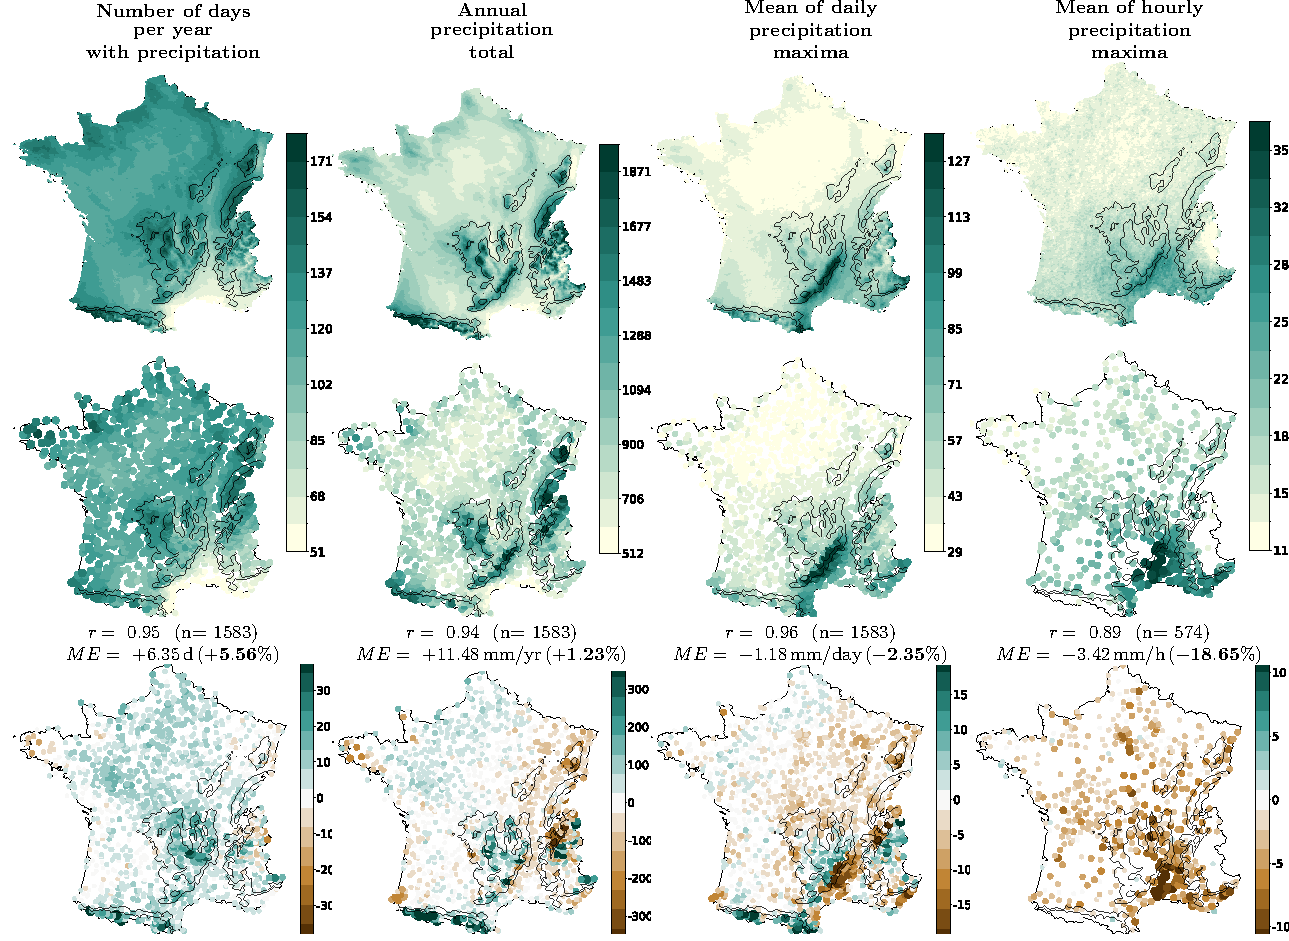
\includegraphics[width=\linewidth]{fig3.pdf}
    \captionsetup{type=figure}
    \setcounter{figure}{2}% prochaine légende = Figure 3
    \caption{\small Climatology between the AROME model (first row), Météo-France stations (second row) with the correlation ($r$) and the number of stations compared (n), and the AROME–Station difference (third row) with the bias ($ME$) and the associated relative deviation (\%) derived from daily data from 1959 to 2022 and hourly data from 1990 to 2022 for a hydrological year.}
\end{center}

Regardless of the indicator (Figure 4), the AROME model faithfully
reproduces observations, with a minimum correlation of 0.64.
Irrespective of the temporal scale---daily (1959--2022 or 1990--2022) or
hourly (1990--2022)---and the season, the simulated fields agree very
well with measured data: correlation ranges from 0.92 to 0.98 for the
number of rainy days and cumulative precipitation. This performance is
maintained for the mean of daily maxima (periods 1959--2022 and
1990--2022) over the hydrological year, autumn, winter, and spring, but
degrades in summer (\textbf{JJA}), with a correlation of 0.85. At the
hourly scale, the quality of the estimation of maxima further
deteriorates: correlation drops by up to 0.3 points, falling to 0.70 in
spring (\textbf{MAM}) and summer (\textbf{JJA}), and to 0.64 in spring
(\textbf{AMJ}). AROME under-represents summer convective extremes,
especially at the hourly scale, despite a well-captured spatial
structure. In April, the bias is +0.22 mm/h (i.e., +3.76\%); in May,
-0.20 mm/h (i.e., -2.42\%) over half of France; and in June, -1.68 mm/h
(i.e., -18.29\%) across all of France. Spatial correlation remains high
in April (\emph{r} = 0.83). \emph{r} = 0.60 in May and 0.63 in June.

\begin{figure}[htp]
\centering
    \includegraphics[width=\textwidth]{fig4.pdf}
    \captionsetup{type=figure}
    \setcounter{figure}{3}% prochaine légende = Figure 4
    \caption{\small Correlations of climatological data between the AROME model and Météo-France stations for each data source.}
\end{figure}

\subsection{Evaluation of Extreme Precipitation
Trends}\label{evaluation-of-extreme-precipitation-trends}

We now assess the trends in decadal return levels (T = 10 years) of
precipitation, visualizing their spatial and seasonal heterogeneity and
quantifying their magnitude and statistical significance in order to
identify the regions and periods where the intensification of extremes
is most pronounced. As before, we begin by analyzing the spatial
distribution of AROME trends in relation to observations. We first
verify that our methodology accurately reproduces the trends already
established at the daily scale over 1959--2022---a long, well-documented
period---in order to validate the signals before moving to the hourly
scale.

The relative \textbf{daily precipitation trends} from 1995 to 2022
estimated with AROME are spatially heterogeneous for the hydrological
year (Figure 5, bottom row). Only the Mercantour region stands out with
a significant increase of between +20\% and +30\%. Stations also show a
generalized positive signal along the Rhône Valley, with trends ranging
from +5\% to \textgreater+30\%. Outside these areas, trends are weak, of
variable sign, and most often not significant, which argues for a
seasonal analysis. In autumn (\textbf{OND}), AROME indicates negative
trends (−10\% to \textless−30\%) over the Paris Basin, the western slope
of the Massif Central, and the Prealps, and a marked increase in the
Mercantour, as previously observed. Stations confirm this pattern, but
with a less pronounced decrease in the Prealps and a clearer signal in
the Alps. The Rhône Valley is notable for increases locally reaching
+40\%. In winter (\textbf{JFM}), AROME highlights marked negative
trends---up to −40\%---in the Verdon and Haut-Var regions; more moderate
decreases (−15\%) also affect the Dordogne Valley, Limousin, and the
northern Massif Central. Conversely, the northern tip of France, the
Jura, and the Vosges show positive trends of +10\% to +30\%. Stations
confirm this pattern, while extending the area of decrease to the
Southern Alps and the French Riviera. In spring (\textbf{AMJ}), the
signal is poorly structured: AROME does not isolate any clear pattern
except for the Camargue coast (\textgreater+30\%). Stations show a
generalized increase over much of France, locally \textgreater+35\%. In
summer (\textbf{JAS}), AROME reveals a generalized decrease across
France, particularly in the southern half, reaching \textless−40\% in
the Pyrénées-Orientales. Stations confirm this spatial pattern,
accentuating it on the French Riviera. Overall, AROME reproduces the
spatial distribution of observed trends, but with low correlation and
sometimes reduced extent, with a mean bias ranging from -0.30\%
(\textbf{JFM}) to -5.44\% (\textbf{AMJ}).

\begin{figure}[htp]
\centering
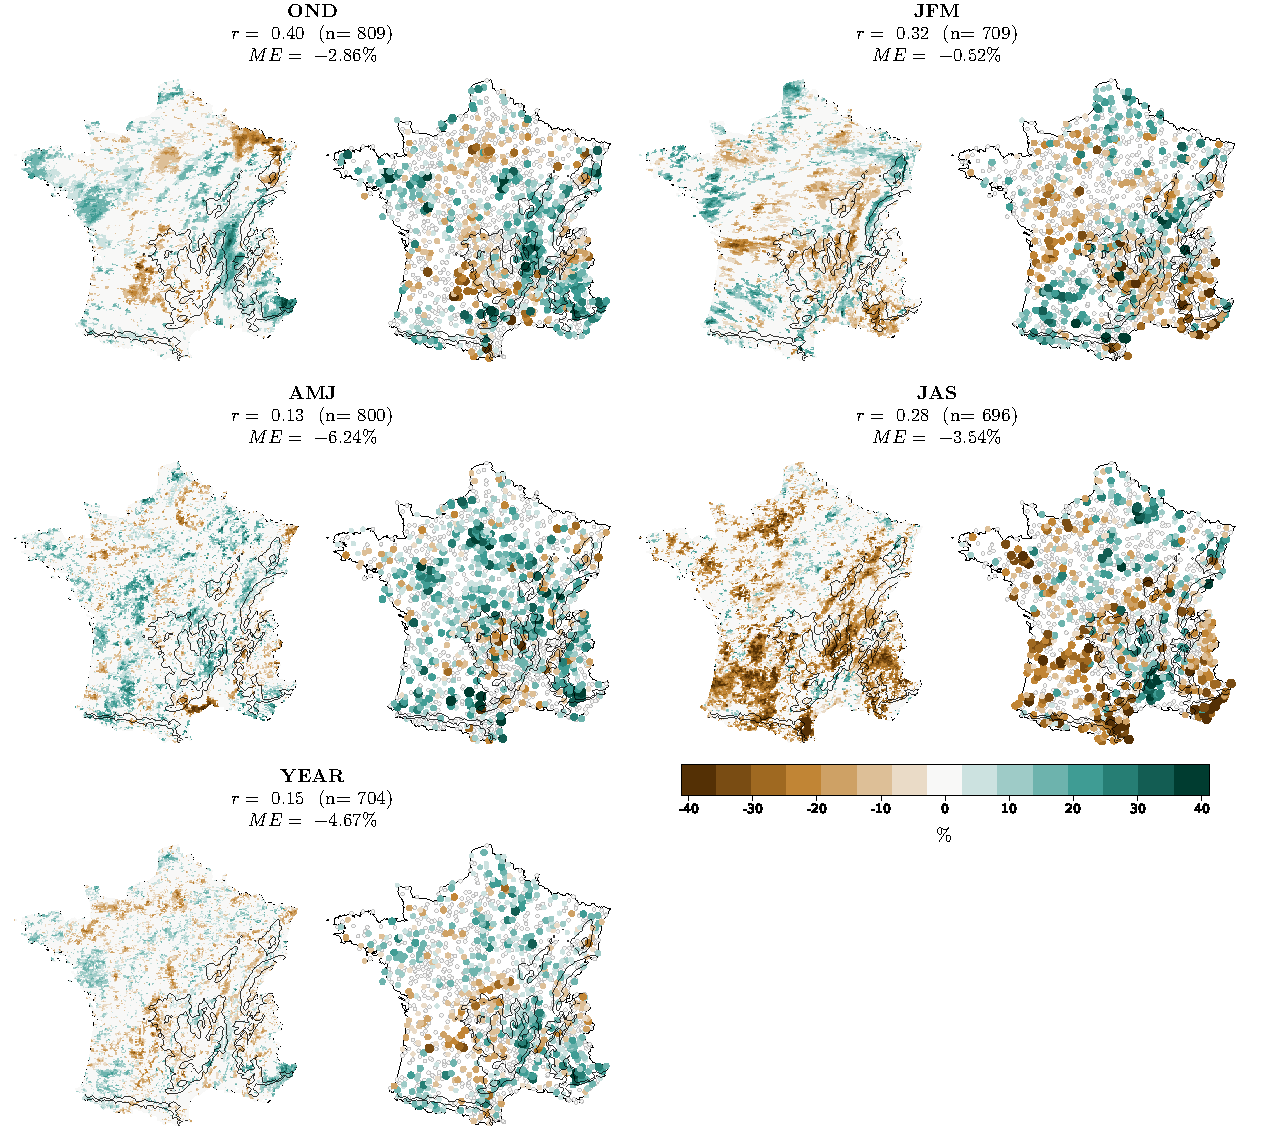
\includegraphics[width=\textwidth]{fig5.pdf}
\end{figure}

Nous passons désormais à l'\textbf{échelle horaire} afin d'évaluer
l'éventuelle intensification des extrêmes infra‑journaliers. Face à
l'hétérogénéité spatiale persistante des tendances saisonnières (Figure
6), nous affinons l'analyse au pas mensuel (Figure 7).

\begin{figure}[htp]
\centering
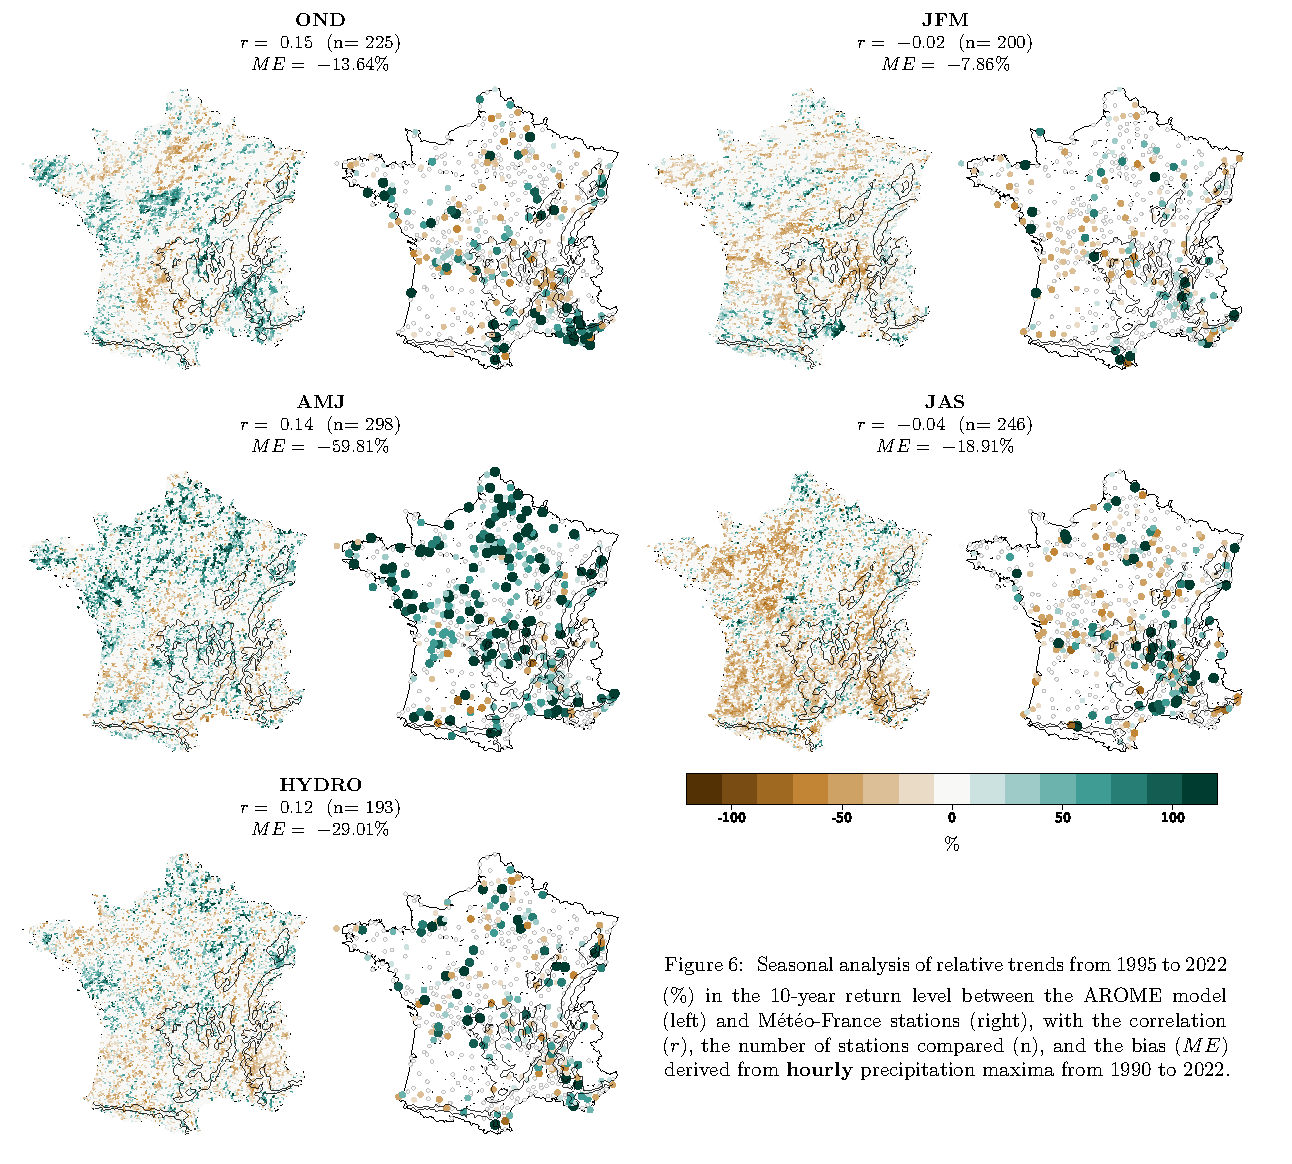
\includegraphics[width=\textwidth]{fig6.pdf}
\end{figure}

AROME indicates positive trends (+25\% to \textgreater+150\%) in the
Rhône Valley and the Prealps in February (\textbf{FEB}), over the
western Mediterranean arc (Roussillon--Lower Languedoc) in March
(\textbf{MAR}), and the eastern arc (Azur Basin) in November
(\textbf{NOV}). Station data confirm this pattern, markedly
strengthening the signal in the Rhône Valley in February, with trends
approximately twice as high as those estimated by AROME. In June
(\textbf{JUN}), both AROME and station data show a predominantly
increasing signal across the entire territory, with local trends
sometimes exceeding +150\%. However, the extremely low spatial
correlation between the two datasets (\emph{r} = 0.10) indicates that,
while the average sign converges, the localization of trends is
inconsistent/noisy. This discrepancy, combined with high summer
convective variability and the short length of monthly series
(1990--2022), calls for caution.

\begin{figure}[htp]
\centering
    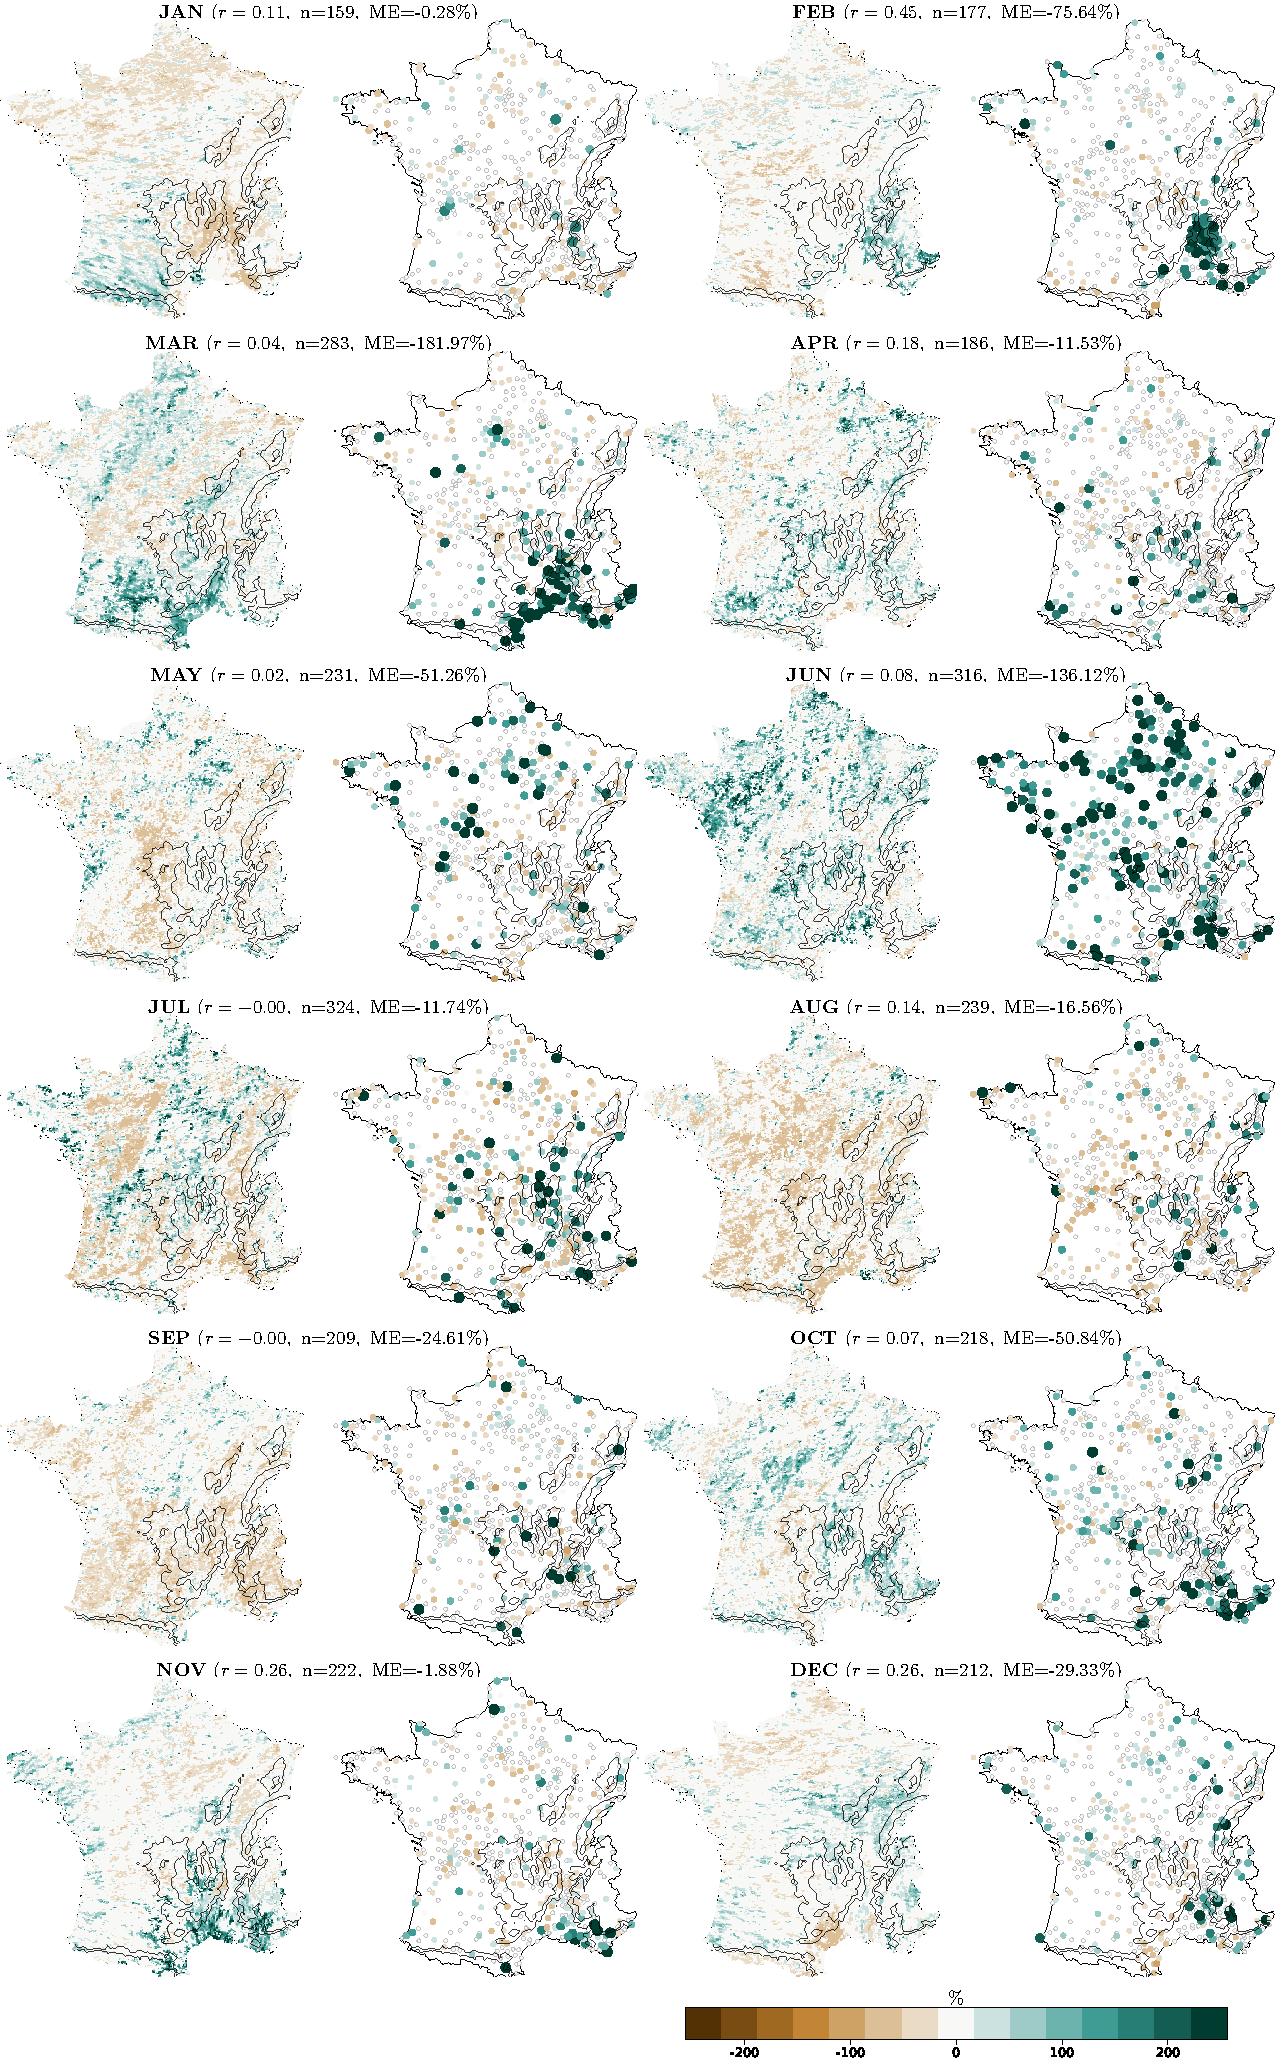
\includegraphics[width=\textwidth]{fig7.pdf}
    \captionsetup{type=figure}
    \setcounter{figure}{6}% prochaine légende = Figure 7
    \captionof{figure}{
        Seasonal analysis of relative trends from 1995 to 2022 (\%) in the 10-year return level
        between the AROME model (left) and Météo-France stations (right), with the correlation ($r$),
        the number of stations compared (n), and the bias ($ME$) derived from hourly precipitation maxima
        from 1990 to 2022.
        }
\end{figure}

To objectify these divergences and assess the robustness of the signals,
we now examine the spatial correlations between AROME and station data,
by season and month, in order to identify where agreement is structural
and where it is mostly noise. At the daily scale (1959--2022), trend
correlations range from 0.14 (\textbf{HYDRO}) to 0.32 (\textbf{OND}) for
seasons and from 0.10 (\textbf{JUN}) to 0.51 (\textbf{DEC}) for months,
with several months reaching or exceeding 0.40 (\textbf{JAN},
\textbf{MAR}, \textbf{AUG}, \textbf{NOV}) (Figure 8). Over the shorter
period (1990--2022), seasonal values span 0.19--0.40 and monthly values
0.02--0.47 (\textbf{JAN} 0.47; \textbf{DEC} 0.35). At the hourly scale
(1990--2022), seasons exhibit weak correlations ranging from 0.00
(\textbf{JAS}) to 0.09 (\textbf{OND}), and monthly correlations extend
from 0.02 (\textbf{SEP}, \textbf{OCT}) to 0.42 (\textbf{FEB}).

When restricting to trends significant by profile likelihood, the daily
scale (1959--2022) shows seasonal correlations from 0.13 (\textbf{AMJ})
to 0.40 (\textbf{OND}) and monthly values from 0.17 (\textbf{JUN}) to
0.77 (\textbf{DEC}), with other months also showing high correlation
(\textbf{JAN} 0.70; \textbf{MAR} 0.71; \textbf{NOV} 0.68; \textbf{AUG}
0.52). For the shorter period (1990--2022), seasonal values range from
0.25 (\textbf{HYDRO}) to 0.52 (\textbf{JFM}) and monthly values from
0.17 (\textbf{JUL}) to 0.69 (\textbf{JAN}), with values above 0.60 in
February, October, and December. At the hourly scale (1990--2022),
seasonal values cover −0.11--0.15 and monthly values −0.01--0.66.
Restricting to significant trends strongly increases daily correlations,
with high monthly maxima. The gain is pronounced in winter and late
summer/autumn (\textbf{JAN}, \textbf{MAR}, \textbf{NOV}, \textbf{DEC},
\textbf{AUG}). At the hourly scale, even after filtering, improvement
remains partial: some months improve (\textbf{FEB}), but several periods
are characterized by correlations near zero or slightly negative
(\textbf{MAY}, \textbf{SEP}).

\begin{figure}[htp]
\centering
    \includegraphics[width=\textwidth]{fig4.pdf}
    \captionsetup{type=figure}
    \setcounter{figure}{7}% prochaine légende = Figure 7
    \caption{\small Correlations of relative trends (all and significant) between AROME and Météo-France stations, by season and by month.}
\end{figure}

\section{Discussion}\label{discussion}

\subsection{Spatial Fidelity of Simulated Climatology and Seasonal
Variability}\label{spatial-fidelity-of-simulated-climatology-and-seasonal-variability}

The results confirm that AROME correctly reproduces the main rainfall
regimes over metropolitan France, as supported by the literature
(Fumière et al. 2020), (Caillaud et al. 2021), (Dura et al. 2024),
(Lucas-Picher et al. 2024). There is an orographic excess over the Alps,
the Pyrenees, and the Massif Central, a marked Atlantic--continental
gradient in the west, and a frequency deficit around the Mediterranean
basin. This consistency with measured reality indicates a satisfactory
representation of dynamic forcings (moisture transport by westerly
flows, orographic uplift, low-level circulation in the Mediterranean).

AROME's ability to reproduce the frequency and quantity of precipitation
is maintained throughout the year, but performance declines for the
average of daily maxima in summer and even more so at the hourly scale.
The model underestimates high-intensity precipitation (\textgreater{} 40
mm/h (Caillaud, Somot, et al. 2021), (Poncet et al. 2024)). Summer
convection remains partially under-resolved despite the 2.5 km spatial
resolution. In this study, we showed (results not shown) that
correlation increases when the time window is extended to 6 or 9 hours.
The model may reproduce the thunderstorm cell starting too late or too
early, spreading intensity over several grid points (not evaluated due
to lack of stations), or underestimating maximum precipitation. The 2--3
km grid spacing is a major step forward for representing convection
without parameterization, but it remains too coarse for applications
sensitive to intense maxima (Prein et al. 2015). It would have been
interesting to include Météo-France's COMEPHORE data (1 km, 15 min) in
this study, but radar reanalyses only begin in 1997, with poor quality
over the Alps before 2007 (Fumière et al. 2020).

\subsection{Trends in Precipitation Extremes: Consistencies,
Divergences, and
Limitations}\label{trends-in-precipitation-extremes-consistencies-divergences-and-limitations}

\textbf{Daily data.} The positive and significant trends are consistent
with the global-scale study of the IPCC (2021), showing an increase in
the 10-year return level. Hotspots in the Mercantour (+20 to +30\%) and,
in terms of stations, in the Rhône Valley (+5 to \textless{} +30\%) are
consistent with work showing an intensification of extremes in
southeastern France and the southern Alps (J. Blanchet, Blanc, et
Creutin 2021). In autumn, an increase in the 20-year return level could
reach the order of magnitude of its mean value in the southeastern Alps.
The marked upward trends of stations (\textgreater{} +35\%) in northern
France echo French projections anticipating stronger increases in daily
extremes in the north under warming (+20\% for +4°C) as shown by
Soubeyroux et al. (2025).

\textbf{Hourly data.} The signals are much less robust at the hourly
scale than at the daily scale. They show very heterogeneous trends,
often weakly or not significant, and sometimes spatially inconsistent
between AROME and stations (in June, \emph{r} = 0.10). This aligns with
the IPCC (2021) finding of low confidence in a global increase in
sub-daily extremes, due to the lack of long, dense, and homogeneous
series. The marked increases in February (Rhône Valley, Pre-Alps), March
(western Mediterranean arc), and November (eastern Mediterranean arc)
are compatible with dynamic and thermo-marine regimes conducive to
Mediterranean/transitional episodes (end of winter, autumn interseason).
The signal doubled by stations in February in the Rhône Valley
highlights AROME's smoothing and amplitude bias for hourly extremes.
However, the restricted period (1990--2022) offers little statistical
power, and interannual convective variability can mask or mimic a trend.
In June, the widespread increase (up to +150\%), but without spatial
agreement between AROME and stations, shows local convective variability
(very localized storms) and errors of point vs.~grid representativeness
become dominant. This is an example of the limits of monthly inference
for convective extremes. It should be noted that this does not result
from an isolated anomaly or a single extreme year. A sensitivity
analysis showed that contrasts persist when the year with the maximum
precipitation is excluded. They therefore reflect a structural signal
linked to the succession of several marked extreme events over the last
decade, reinforcing recent trends rather than a punctual temporal
artifact.

Regional studies highlight sub-daily sensitivities of +7 to +13\%/°C,
sometimes exceeding Clausius--Clapeyron, especially for brief convective
storms (Molnar et al. 2015). This study does not identify a clear signal
with the AROME model, which strongly underestimates hourly peaks, while
stations capture local spikes. This was expected given that the
Clausius--Clapeyron-related trend in extremes should theoretically be
half as strong as the observed trends.

\subsection{Statistical Robustness of
Signals}\label{statistical-robustness-of-signals}

A long window (1959--2022) reduces estimation uncertainties and samples
several climate regimes (global dimming phase dominated by aerosols
until the 1980s, then accelerated warming from the late 1980s--1990s).
This mixing of regimes mechanically attenuates the average slope: part
of the recent signal is drowned in multidecadal variability. Conversely,
a short window (1990--2022) isolates the regime dominated by rapid
warming, the decrease in sulfate aerosols in Europe, and the
quasi-linear increase in water vapor content (+7\%/°C), which brings out
clearer positive trends. The two diagnostics are therefore complementary
and must be interpreted separately to avoid confusing multidecadal noise
with long-term anthropogenic forcing.

As a first approximation, the monthly distributions of relative trends
in the 10-year return level are centered on 0\% over 1959--2022, while
1990--2022 shows a slight shift toward increases, especially in spring
and early winter, in line with the literature on the recent
amplification of daily extremes. Even though breakpoints were allowed
when justified by the LRT, the gradual transition (about 10 years)
between the dimming era and the post-1985 warm regime remains partly
absorbed by long-window models, reducing the average slope compared to
short-window models that fit the recent quasi-linear portion. This
explains, for example, the observed national average trend of −1.6\%
over 1959--2022 versus +3.5\% over 1990--2022.

These differences are also expected from a statistical point of view:
DeGaetano et Castellano (2018) shows that, for trends \textgreater{}
0.5\%/year in the location parameter μ, reducing the window from 60 to
30 years can change the estimated slope of decadal return levels by 10
to 20\%. In other words, the length of the window and the
(non-)stationarity of the climate strongly influence trend estimation,
even when breakpoints detected by LRT are integrated.

\subsection{Regional Signals}\label{regional-signals}

\textbf{Filtering strengthens consistency, but AROME struggles with fine
extremes.} By retaining only significant trends, many sites where the
signal is dominated by climate noise are eliminated, improving the
spatial consistency of trends and thus regional diagnostics. At the
daily scale, monthly correlation values between AROME and stations range
from 0.40 to 0.77 after filtering for significance, compared to less
than 0.20 at the hourly scale. This jump could be related to AROME's
difficulty in explaining fine convective maxima at the hourly scale.

The seasonal breakdown highlights a hierarchy dominated by winter, which
systematically concentrates the strongest correlations and moderate to
marked increases in return levels. In winter, precipitation in western
Europe comes from Atlantic disturbances carried by westerly flows. Their
intensity depends directly on the amount of water vapor in these air
masses, which increases with temperature according to the
Clausius--Clapeyron law. This is why milder winters can sometimes be
wetter, even with identical atmospheric dynamics. Spring and early
summer, by contrast, show systematic minima in correlation. This reveals
the persistent difficulty, even at 2.5 km resolution, in representing
weakly organized convection typical of this season. Diurnal warming
mainly triggers isolated local storms. The influence of Atlantic
disturbances decreases, as the jet stream and its frontal systems move
northward. Vertical wind shear weakens, preventing the organization of
storms into durable structures. The result is brief, highly localized,
and poorly structured precipitation that the simulation--observation
pair still captures poorly. In August and September, the relative
convergence of distributions (close medians and correlations \textless{}
0.20) reflects high variability and a shared contribution between
continental thunderstorm episodes and early Mediterranean systems. The
mix of rainfall mechanisms reduces consistency between sites and AROME's
ability to reproduce the seasonality of trends.

\textbf{The Rhône Valley} appears to be a ``hotspot'' for positive
trends in return levels, consistent with the resurgence of Cévenol
events in autumn and enhanced orographic disturbances in southerly flows
(Fresnay et al. 2012). AROME under-diagnoses these increases but
reproduces their location, suggesting that the dynamics (meridional
channeling and orographic uplift) are correctly simulated, while
convective intensity remains under-resolved. Ribes et al. (2019)
highlights that this area accumulates the strongest observed
intensification in the entire Mediterranean south, with a mean intensity
gain of +22\% in daily extreme precipitation between 1961 and 2015. They
show, in the southeastern half (including Gard, Ardèche, and Drôme), a
doubling of the frequency of events \textgreater200 mm in 24 hours since
1985, with most associated with hourly peaks \textgreater50 mm. J.
Blanchet, Blanc, et Creutin (2021) show that, since the 1980s, the
autumn Mediterranean influence has clearly intensified and advanced in
the season, with the strongest increases in return levels centered on
the Rhône--Alps corridor and the Cévennes. This ``hotspot'' is striking
at the national scale for hourly data in February. Since the early
1990s, the average winter temperature in France has increased by +0.8°C
(difference between the 1961--1990 and 1991--2020 Météo-France
normals)---i.e., an additional moisture retention capacity of about +6\%
according to the Clausius--Clapeyron relation. Three mechanisms could
combine in February: 1) rain replaces snow, concentrating the water
column (Zaqout et Andradóttir 2024); 2) there are slopes of 12\%/°C for
hourly extremes when T = 0--8°C---almost double the classic 7\%
(Drobinski et al. 2016); and 3) more humid southerly flows inject more
vapor into a very efficient orographic corridor (Lorente‐Plazas et al.
2020).

\section{Conclusion}\label{conclusion}

This study presents the first comprehensive evaluation of the AROME
regional climate model (2.5 km resolution, 1959--2022), forced by ERA5,
to reproduce precipitation extremes in France at both daily and hourly
scales. By cross-referencing model simulations with dense observations
from Météo-France's network, this work addresses a critical scientific
gap: the characterization of sub-daily extreme precipitation trends,
which are essential for managing flash flood and severe storm risks.

\textbf{Key findings.} Our analyses confirm that the AROME model
accurately reproduces France's major rainfall regimes, with high spatial
correlation for daily indicators (frequency, cumulative totals, maxima).
However, the representation of hourly extremes remains limited,
particularly in summer, where weakly organized convection is
under-resolved at 2.5 km. Systematic biases---such as the
underestimation of intense peaks and the smoothing of convective
events---highlight the need for even finer resolution to capture local
thunderstorm variability.

The analysis of decadal return level trends reveals a marked
intensification of daily extremes in southeastern France (Rhône Valley,
Mercantour, Cévennes), consistent with climate projections and
Clausius--Clapeyron scaling. At the hourly scale, signals are more
heterogeneous and less robust, with significant increases in February,
March, and November, but high spatial variability and low
model-observation correlation in summer. Filtering for statistically
significant trends improves agreement, especially in winter and autumn,
but hourly convective extremes remain poorly simulated in spring and
summer due to the complexity of physical mechanisms and the short
duration of available time series.

\textbf{Implications and perspectives.} This study underscores the added
value of explicit-convection models for extreme precipitation research,
while also exposing their limitations for convective events at
resolutions coarser than 1 km. The Rhône Valley is confirmed as a
``hotspot'' for the intensification of hourly extremes, driven by
increased moisture flux, orographic enhancement, and the winter
rain-snow transition. These findings provide actionable insights for
adapting territories to hydrometeorological risks, particularly through
improved early warning systems and urban planning.

To build on this work, integrating very high-resolution radar data (1
km, 15 min) could refine the validation of convective extremes, and
exploring future climate scenarios would help anticipate risk evolution.
Furthermore, developing hybrid models that combine dynamic simulations
with statistical approaches could enhance the representation of
fine-scale extremes, especially in complex terrain.

In conclusion, this research establishes a robust foundation for
understanding and managing precipitation extremes in France amid
accelerating climate change. It paves the way for more targeted studies
that integrate both modeling advances and the operational needs of risk
prevention stakeholders.

\section*{References}\label{references}
\addcontentsline{toc}{section}{References}

\phantomsection\label{refs}
\begin{CSLReferences}{1}{0}
\bibitem[\citeproctext]{ref-Berghald2025}
Berghald, Sebastian, Juliette Blanchet, Antoine Blanc, et David Penot.
2025. {«~Climatology and trends of observed daily and hourly extreme
precipitation in the French Alps~»}. \emph{EGUsphere {[}preprint{]}}.
\url{https://doi.org/10.5194/egusphere-2025-3073}.

\bibitem[\citeproctext]{ref-Blanc2024}
Blanc, A., C. Misset, R. Mainieri, et B. Llamas. 2024. {«~{Rétro-analyse
de la crue du torrent des Etançons du 21 juin 2024}~»}. Tech. rep. RTM
de l'Isère et Département Risques Naturels -- Pôle RTM.

\bibitem[\citeproctext]{ref-blanchet2021explaining}
Blanchet, J., A. Blanc, et J.-D. Creutin. 2021. {«~Explaining recent
trends in extreme precipitation in the Southwestern Alps by changes in
atmospheric influences~»}. \emph{Weather and Climate Extremes} 33:
100356. \url{https://doi.org/10.1016/j.wace.2021.100356}.

\bibitem[\citeproctext]{ref-Blanchet2018}
Blanchet, Juliette, Gilles Molinié, et Julien Touati. 2018. {«~Spatial
analysis of trend in extreme daily rainfall in southern France~»}.
\emph{Climate Dynamics} 51 (3): 799‑812.
\url{https://doi.org/10.1007/s00382-016-3122-7}.

\bibitem[\citeproctext]{ref-caillaud2021simulation}
Caillaud, C. et al. 2021. {«~Simulation using CNRM-AROME46t1 (2.5km)
CP-RCM performed by CNRM~»}. \emph{Climate Dynamics}.
\url{https://doi.org/10.1007/s00382-020-05558-y}.

\bibitem[\citeproctext]{ref-Caillaud2021}
Caillaud, C., S. Somot, A. Alias, et et al. 2021. {«~Modelling
Mediterranean heavy precipitation events at climate scale: an
object-oriented evaluation of the CNRM-AROME convection-permitting
regional climate model~»}. \emph{Climate Dynamics} 56: 1717‑52.
\url{https://doi.org/10.1007/s00382-020-05558-y}.

\bibitem[\citeproctext]{ref-arome2014}
Centre National de Recherches Météorologiques. 2014. {«~AROME en
bref~»}. Météo-France, UMR 3589 CNRM.
\url{https://www.umr-cnrm.fr/spip.php?article120&id_document=1077}.

\bibitem[\citeproctext]{ref-clapeyron1834}
Clapeyron, Émile. 1834. {«~Mémoire sur la puissance motrice de la
chaleur~»}. \emph{Journal de l'École polytechnique} 23: 153‑91.
\url{https://gallica.bnf.fr/ark:/12148/bpt6k4336792/f179.image}.

\bibitem[\citeproctext]{ref-cnrm_arome2007}
CNRM--Météo‐France. 2007. {«~AROME: modèle opérationnel à maille
convectionnelle~»}. Document PDF, UMR--CNRM.
\url{https://www.umr-cnrm.fr/IMG/pdf/arome2007.pdf}.

\bibitem[\citeproctext]{ref-coles2001introduction}
Coles, Stuart. 2001. \emph{An Introduction to Statistical Modeling of
Extreme Values}. Springer Series in Statistics. London: Springer.

\bibitem[\citeproctext]{ref-ecmwf_era5_data_documentation}
Copernicus Climate Change Service (C3S), et European Centre for
Medium-Range Weather Forecasts (ECMWF). 2025. {«~ERA5: data
documentation~»}. ECMWF Copernicus Knowledge Base.
\url{https://confluence.ecmwf.int/display/CKB/ERA5\%3A+data+documentation}.

\bibitem[\citeproctext]{ref-DeGaetano2018}
DeGaetano, Arthur T., et Christopher M. Castellano. 2018. {«~Selecting
Time Series Length to Moderate the Impact of Nonstationarity in Extreme
Rainfall Analyses~»}. \emph{Journal of Applied Meteorology and
Climatology} 57 (10): 2285‑96.
\url{https://doi.org/10.1175/JAMC-D-18-0046.1}.

\bibitem[\citeproctext]{ref-Donat2013}
Donat, M. G., L. V. Alexander, H. Yang, I. Durre, R. Vose, R. J. H.
Dunn, K. M. Willett, et al. 2013. {«~Updated Analyses of Temperature and
Precipitation Extreme Indices Since the Beginning of the Twentieth
Century: The HadEX2 Dataset~»}. \emph{Journal of Geophysical Research:
Atmospheres} 118 (5): 2098‑118.
\url{https://doi.org/10.1002/jgrd.50150}.

\bibitem[\citeproctext]{ref-Donat2016}
Donat, Markus G., Andrew L. Lowry, Lisa V. Alexander, Paul A. O'Gorman,
et Nicola Maher. 2016. {«~More extreme precipitation in the world's dry
and wet regions~»}. \emph{Nature Climate Change} 6 (5): 508‑13.
\url{https://doi.org/10.1038/nclimate2941}.

\bibitem[\citeproctext]{ref-Drobinski2016}
Drobinski, Philippe, Bastien Alonzo, Sophie Bastin, Nicolas Da Silva, et
Caroline J. Muller. 2016. {«~Scaling of precipitation extremes with
temperature in the French Mediterranean region: What explains the hook
shape?~»} \emph{Journal of Geophysical Research: Atmospheres} 121 (7):
3100‑3119. \url{https://doi.org/10.1002/2015JD023497}.

\bibitem[\citeproctext]{ref-hess-28-2579-2024}
Dura, V., G. Evin, A.-C. Favre, et D. Penot. 2024. {«~Spatial
variability in the seasonal precipitation lapse rates in complex
topographical regions -- application in France~»}. \emph{Hydrology and
Earth System Sciences} 28 (12): 2579‑2601.
\url{https://doi.org/10.5194/hess-28-2579-2024}.

\bibitem[\citeproctext]{ref-Fresnay2012}
Fresnay, S., A. Hally, C. Garnaud, E. Richard, et D. Lambert. 2012.
{«~Heavy precipitation events in the Mediterranean: sensitivity to cloud
physics parameterisation uncertainties~»}. \emph{Natural Hazards and
Earth System Sciences} 12: 2671‑88.
\url{https://doi.org/10.5194/nhess-12-2671-2012}.

\bibitem[\citeproctext]{ref-Fumiere2020}
Fumière, Quentin, Michel Déqué, Olivier Nuissier, Samuel Somot,
Antoinette Alias, Cécile Caillaud, Olivier Laurantin, et Yann Seity.
2020. {«~Extreme rainfall in Mediterranean France during the fall: added
value of the CNRM-AROME Convection-Permitting Regional Climate Model~»}.
\emph{Climate Dynamics} 55: 77‑91.
\url{https://doi.org/10.1007/s00382-019-04898-8}.

\bibitem[\citeproctext]{ref-IPCC2021}
IPCC. 2021. \emph{Climate Change 2021: The Physical Science Basis}.
Cambridge, UK: Cambridge University Press.
\url{https://doi.org/10.1017/9781009157896}.

\bibitem[\citeproctext]{ref-IPCC_2022_WGIII}
---------. 2022. \emph{Climate Change 2022: Mitigation of Climate
Change. Contribution of Working Group III to the Sixth Assessment Report
of the Intergovernmental Panel on Climate Change}. Cambridge, UK; New
York, NY, USA: Cambridge University Press.
\url{https://doi.org/10.1017/9781009157926}.

\bibitem[\citeproctext]{ref-LorentePlazas2020}
Lorente‐Plazas, Raquel, Juan Pedro Montávez, Ana María Ramos, Sara
Jerez, Ricardo M. Trigo, et Pedro Jiménez‐Guerrero. 2020. {«~Unusual
Atmospheric‑River‑Like Structures Coming From Africa Induce Extreme
Precipitation Over the Western Mediterranean Sea~»}. \emph{Journal of
Geophysical Research: Atmospheres} 125 (e2019JD031280).
\url{https://doi.org/10.1029/2019JD031280}.

\bibitem[\citeproctext]{ref-LucasPicher2024}
Lucas-Picher, P., E. Brisson, C. Caillaud, et al. 2024. {«~Evaluation of
the convection-permitting regional climate model CNRM-AROME41t1 over
Northwestern Europe~»}. \emph{Climate Dynamics} 62: 4587‑4615.
\url{https://doi.org/10.1007/s00382-022-06637-y}.

\bibitem[\citeproctext]{ref-meteofrance}
Météo-France. 2010. \emph{{La météorologie}}. 2e édition. {Paris,
France}: {Éditions Eyrolles}.

\bibitem[\citeproctext]{ref-meteo-france_2020_breve_observation_classique}
---------. 2020. {«~Une brève histoire de l'observation~»}.
\url{https://meteofrance.com/magazine/meteo-histoire/observation/une-breve-histoire-de-lobservation}.

\bibitem[\citeproctext]{ref-MeteoFrance2024_episodesArdeches}
---------. 2024a. {«~{Bilan climatique de l'année 2024\,: France
hexagonale et Corse}~»}. \{Rapport\}. {Météo-France}.
\url{https://meteofrance.fr/sites/meteofrance.fr/files/files/editorial/Bilan_annee_2024_France_hexagonale-et-Corse.pdf}.

\bibitem[\citeproctext]{ref-meteofrance2024}
---------. 2024b. {«~Données d'observations météorologiques issues des
stations synoptiques et climatologiques~»}. Open Data on data.gouv.fr.
\url{https://www.data.gouv.fr/fr/datasets/donnees-dobservations-meteorologiques-issues-des-stations-synoptiques-et-climatologiques/}.

\bibitem[\citeproctext]{ref-MeteoFrance2025}
---------. 2025. {«~{Retour sur les violents orages dans le sud du
pays}~»}.
\url{https://meteofrance.com/actualites-et-dossiers/actualites/retour-sur-les-violents-orages-dans-le-sud-du-pays}.

\bibitem[\citeproctext]{ref-meteofrance2024_episodesMediterraneens}
Météo‑France. 2024. {«~Quel est l'impact du changement climatique sur
les épisodes méditerranéens\,?~»}
\url{https://meteofrance.com/le-changement-climatique/quel-climat-futur/quel-est-limpact-du-changement-climatique-sur-les}.

\bibitem[\citeproctext]{ref-molnar2015relation}
Molnar, P. et al. 2015. {«~Relation of intense rainstorm properties to
temperature~»}. \emph{Hydrology and Earth System Sciences} 19: 1753‑66.

\bibitem[\citeproctext]{ref-ogorman2015contrasting}
O'Gorman, P. A. 2015. {«~Contrasting responses of mean and extreme
precipitation to climate change~»}. \emph{Current Climate Change
Reports} 1 (2): 79‑92. \url{https://doi.org/10.1038/nature13625}.

\bibitem[\citeproctext]{ref-poncet2024convection}
Poncet, Nils, Philippe Lucas‑Picher, Yves Tramblay, Guillaume Thirel,
Humberto Vergara, Jonathan Gourley, et Antoinette Alias. 2024. {«~Does a
convection‑permitting regional climate model bring new perspectives on
the projection of Mediterranean floods?~»} \emph{Natural Hazards and
Earth System Sciences} 24 (4): 1163‑83.
\url{https://doi.org/10.5194/nhess-24-1163-2024}.

\bibitem[\citeproctext]{ref-Prein2015Review}
Prein, Andreas F., Wolfgang Langhans, Giorgia Fosser, Andrew Ferrone,
Nikolina Ban, Klaus Goergen, Michael Keller, et al. 2015. {«~A Review on
Regional Convection‐Permitting Climate Modeling: Demonstrations,
Prospects, and Challenges~»}. \emph{Reviews of Geophysics} 53 (2):
323‑61. \url{https://doi.org/10.1002/2014RG000475}.

\bibitem[\citeproctext]{ref-Ribes2019}
Ribes, A., S. Thao, R. Vautard, B. Dubuisson, S. Somot, J. Colin, S.
Planton, et J. M. Soubeyroux. 2019. {«~Observed increase in extreme
daily rainfall in the French Mediterranean~»}. \emph{Climate Dynamics}
52: 1095‑1114. \url{https://doi.org/10.1007/s00382-018-4179-2}.

\bibitem[\citeproctext]{ref-soubeyroux:hal-04991790}
Soubeyroux, Jean-Michel, Sébastien Bernus, Brigitte Dubuisson, Agathe
Drouin, Thumette Madec, Fabienne Rousset, Raphaëlle Samacoïts, et al.
2025. {«~{{À} quel climat s'adapter en France selon la TRACC ? partie
2}~»}. {Meteo-France}. \url{https://hal.science/hal-04991790}.

\bibitem[\citeproctext]{ref-Soubeyroux01022015}
Soubeyroux, Jean-Michel, Luc Neppel, Jean-Michel Veysseire, Yves
Tramblay, Julie Carreau, et Viviane Gouget. 2015. {«~Evolution des
précipitations extrêmes en France en contexte de changement
climatique~»}. \emph{La Houille Blanche} 101 (1): 27‑33.
\url{https://doi.org/10.1051/lhb/2015004}.

\bibitem[\citeproctext]{ref-wmo2024}
World Meteorological Organization (WMO). 2025. {«~State of the Global
Climate 2024~»}.
\url{https://public.wmo.int/en/our-mandate/climate/wmo-statement-state-of-global-climate}.

\bibitem[\citeproctext]{ref-ZAQOUT2024131439}
Zaqout, Tarek, et Hrund Ólöf Andradóttir. 2024. {«~Impacts of climate
change on winter flood mechanisms: Spatial variability, trends, and
bivariate frequency of rain-on-snow and soil frost~»}. \emph{Journal of
Hydrology} 638: 131439.
https://doi.org/\url{https://doi.org/10.1016/j.jhydrol.2024.131439}.

\end{CSLReferences}

\end{document}